\documentclass[final]{book}
\newcommand{\doctitle}{HSA Runtime Programmer's Reference Manual}
\newcommand{\docversion}{0.187}

% Needed so characters such as underscore are recognized in PDF
% viewers. Otherwise searching for say `hsa_open` produces no
% results
\usepackage[T1]{fontenc}

\usepackage[top=2.5cm,bottom=2.5cm,left=2.5cm,right=2.5cm]{geometry}

\usepackage[toc,page]{appendix}
\usepackage[usenames,dvipsnames,svgnames,table]{xcolor}
  \definecolor{lightgray}{gray}{0.94}
\usepackage{makeidx}
\usepackage[final]{graphicx}
\usepackage{pbox}
\usepackage{sidecap}
\usepackage{float}

% overwrite global draft option so the source is shown in draft mode
\usepackage[final]{listings}

% allow tables across page breaks
\usepackage{longtable}

% Use Tikz for simple diagrams
\usepackage{tikz}
\usetikzlibrary{arrows,automata,positioning,chains}
\tikzset{
    % define global arrow tip format
    >=angle 45}

% allows width arithmetic, currently used in the LaTeX generated by xml2tex
\usepackage{calc}
% allow usage of underscore w/o resorting to underscore package
% the underscore package imposes more restrictions on where underscores still
% cannot be used (e.g.: labels)
\catcode`\_=12

\usepackage{ifthen}
\usepackage{textcomp}

% inline enumerations and itemizes in the paragraph instead of breaking
\usepackage{paralist}

% Customizable headers/footers
\usepackage{fancyhdr}

% add API index. Note that 'imakeidx' works within Latex (unlike 'makeidx', which
% requires running 'makeindex' from command line)
\usepackage{imakeidx}
\makeindex[name=api,title=Index - Core APIs,columns=1,intoc]
\makeindex[name=ext,title=Index - Extension APIs,columns=1,intoc]

% Times font definitions
\usepackage{times}

% allows customization of description environment (margin, indentation, etc.)
\usepackage{enumitem}

\lstset{% in alphabetical order
        backgroundcolor=\color{lightgray},
        basicstyle=\footnotesize,
        breakatwhitespace=true,
        breaklines=true,
        captionpos=b,      % sets the caption-position to bottom
        columns=fullflexible,
        commentstyle=\color{ForestGreen},
        emphstyle={\textbf},
        frame=single,
        framexbottommargin=3pt, % bottom frame padding
        framextopmargin=3pt, % top frame padding
        inputencoding=utf8,
        keywordstyle=\color{blue},
        language=C,
        rulecolor=\color{lightgray}, % invisible (we use it because it allows padding)
        showstringspaces=false,
        tabsize=4,
}
% Use Example instead of Listing in captions
\renewcommand{\lstlistingname}{Example}
% List of Listings -> List of Examples
\renewcommand{\lstlistlistingname}{List of \lstlistingname s}
% include automatically-generated Listing commands
\input{api/altlatex/listings}

% formatting of arguments, function names, types, etc.
% remember to add this commands to the safe command list of Latexdiff so
% it includes them in the diff algorithm
\newcommand{\hsaarg}[1]{\textit{#1}}
\newcommand{\reffun}[1]{\textbf{#1}}
\newcommand{\refarg}[1]{\textit{#1}}
\newcommand{\reffld}[1]{\textit{#1}}
\newcommand{\reftyp}[1]{#1}
\newcommand{\refenu}[1]{\reftyp{#1}}
\newcommand{\refhsl}[1]{\reffun{#1}}

% allows string comparison, which is used to match \hsaref arguments
\usepackage{pdftexcmds}
% Automatically generated file containing all the definitions in the header that
% can be referenced via \hsaref commands
\input{api/altlatex/commands}

% every section in a new page
\usepackage{etoolbox}
\pretocmd{\section}{%
  \ifnum\value{section}=0 \else\clearpage\fi
}{}{}

% define marginparwidth so todonotes renders properly
\setlength{\marginparwidth}{2cm}
\usepackage[obeyDraft,obeyFinal,textsize=scriptsize]{todonotes}

\usepackage[final, % use links even if the document is draft
            linktoc=all,  % sections and subsections linked
            colorlinks=true, % just in case we want to color links in future
            allcolors=black,
            unicode
           ]{hyperref}

% alternate rowcolors for all long-tables
\let\oldlongtable\longtable
\let\endoldlongtable\endlongtable
\newenvironment{mylongtable}{\rowcolors{0}{lightgray}{lightgray}\longtable} {
\endlongtable}

% Alter some LaTeX defaults for better treatment of figures:
% See p.105 of "TeX Unbound" for suggested values.
% See pp. 199-200 of Lamport's "LaTeX" book for details.
%   General parameters, for ALL pages:
\renewcommand{\topfraction}{0.9}	% max fraction of floats at top
\renewcommand{\bottomfraction}{0.8}	% max fraction of floats at bottom
%   Parameters for TEXT pages (not float pages):
\setcounter{topnumber}{2}
\setcounter{bottomnumber}{2}
\setcounter{totalnumber}{4}     % 2 may work better
\setcounter{dbltopnumber}{2}    % for 2-column pages
\renewcommand{\dbltopfraction}{0.9}	% fit big float above 2-col. text
\renewcommand{\textfraction}{0.07}	% allow minimal text w. figs
%   Parameters for FLOAT pages (not text pages):
\renewcommand{\floatpagefraction}{0.7}	% require fuller float pages
% N.B.: floatpagefraction MUST be less than topfraction !!
\renewcommand{\dblfloatpagefraction}{0.7}	% require fuller float pages

% push footer a little further away
\setlength{\footskip}{35pt}

% Side notes. One command per author
\newcommand{\mariotodo}[1]{\todo[color=CarnationPink]{#1}}

% Increase paragraph separation
\setlength{\parskip}{2mm}

% no indentation
\setlength{\parindent}{0cm}

% number (sub)sections up to level 3
\setcounter{secnumdepth}{3}

\makeindex
\setcounter{tocdepth}{3}
\renewcommand{\footrulewidth}{0.4pt}
\renewcommand{\familydefault}{\sfdefault}

\RequirePackage[normalem]{ulem} %DIF PREAMBLE
\newenvironment{DIFnomarkup}{}{}

% header and footer layout
\newcommand{\hfstyle}{
\fancyhf{} % clear all header and footer fields
\fancyfoot[LE,RO]{\scriptsize{\thepage}}
\fancyfoot[LO,RE]{\scriptsize{\doctitle$\:$v\docversion $\:$-$\:$\today}}
\fancyhead[RE]{\scriptsize{\nouppercase{\leftmark}}}
\fancyhead[LO]{\scriptsize{\nouppercase{\rightmark}}}
\renewcommand{\headrulewidth}{0pt}
\renewcommand{\footrulewidth}{0pt}
}

% avoid vertical spacing in order to get a fixed-size page
%\hfuzz=20pt
%\vfuzz=20pt
%\hbadness=2000
%\vbadness=\maxdimen
%\raggedbottom
%\setlength{\emergencystretch}{1mm}
%\fussy

\pagestyle{fancy}
\renewcommand{\chaptermark}[1]{\markboth{#1}{}}
\renewcommand{\sectionmark}[1]{\markright{#1}{}}
\hfstyle{}

% plain style is identical to fancy style. This avoids different formatting in
% the first page of every chapter, for example.
\fancypagestyle{plain}{\hfstyle{}}

\begin{document}

\pagenumbering{roman}
\addcontentsline{toc}{chapter}{Cover} % add cover to TOC

\begin{titlepage}

\includegraphics[width=.4\textwidth]{fig/foundation_small.png}
\vspace*{7cm}
\begin{center}
{\Large \doctitle\\[1ex]\large\docversion}\\
\vspace*{1cm}
\vspace*{0.5cm}
{\small \today}\\
\vspace*{0.5cm}
{\small Draft}\\
\end{center}
\end{titlepage}
\thispagestyle{empty} {\textcopyright 2013-2014 HSA Foundation. All rights
  reserved.}


The contents of this document are provided in connection with the HSA Foundation
specifications. This specification is protected by copyright laws and contains
material proprietary to the HSA Foundation. It or any components may not be
reproduced, republished, distributed, transmitted, displayed, broadcast or
otherwise exploited in any manner without the express prior written permission
of HSA Foundation. You may use this specification for implementing the
functionality therein, without altering or removing any trademark, copyright or
other notice from the specification, but the receipt or possession of this
specification does not convey any rights to reproduce, disclose, or distribute
its contents, or to manufacture, use, or sell anything that it may describe, in
whole or in part.

HSA Foundation grants express permission to any current Founder, Promoter,
Supporter Contributor, Academic or Associate member of HSA Foundation to copy
and redistribute UNMODIFIED versions of this specification in any fashion,
provided that NO CHARGE is made for the specification and the latest available
update of the specification for any version of the API is used whenever
possible. Such distributed specification may be re-formatted AS LONG AS the
contents of the specification are not changed in any way. The specification may
be incorporated into a product that is sold as long as such product includes
significant independent work developed by the seller. A link to the current
version of this specification on the HSA Foundation web-site should be included
whenever possible with specification distributions.

HSA Foundation makes no, and expressly disclaims any, representations or
warranties, express or implied, regarding this specification, including, without
limitation, any implied warranties of merchantability or fitness for a
particular purpose or non-infringement of any intellectual property. HSA
Foundation makes no, and expressly disclaims any, warranties, express or
implied, regarding the correctness, accuracy, completeness, timeliness, and
reliability of the specification. Under no circumstances will the HSA
Foundation, or any of its Founders, Promoters, Supporters, Academic,
Contributors, and Associates members or their respective partners, officers,
directors, employees, agents or representatives be liable for any damages,
whether direct, indirect, special or consequential damages for lost revenues,
lost profits, or otherwise, arising from or in connection with these materials.

\clearpage
\phantomsection
\addcontentsline{toc}{chapter}{Contents} % add TOC to TOC
\tableofcontents

\clearpage
\pagenumbering{arabic}
\setcounter{page}{1}

\chapter{Introduction} \label{index}
\section{Overview}\label{overview}

Recent heterogeneous system designs have integrated CPU, GPU, and other
accelerator devices into a single platform with a shared high-bandwidth memory
system.  Specialized accelerators now complement general purpose CPU chips and
are used to provide both power and performance benefits.  These
heterogeneous designs are now widely used in many computing markets including
cellphones, tablets, personal computers, and game consoles. The Heterogeneous
System Architecture (HSA) builds on the close physical integration of
accelerators that is already occurring in the marketplace, and takes the next
step by defining standards for uniting the accelerators architecturally. The HSA
specifications include requirements for virtual memory, memory coherency,
architected dispatch mechanisms, and power-efficient signals. HSA refers to
these accelerators as "components".

The HSA system architecture defines a consistent base for building portable
applications that access the power and performance benefits of the dedicated HSA
components. Many of these components, including GPUs and DSPs, are capable and
flexible processors that have been extended with special hardware for
accelerating parallel code. Historically these devices have been difficult to
program due to a need for specialized or proprietary programming languages. HSA
aims to bring the benefits of these components to mainstream programming
languages using similar or identical syntax to that which is provided for
programming multi-core CPUs. For more information on the system architecture,
refer to the HSA Platform System Architecture Specification, version 1.0
'Provisional Ratified'~\cite{sar}.

In addition to the system architecture, HSA defines a portable, low-level,
compiler intermediate language called ``HSAIL''.  A high-level compiler
generates the HSAIL for the parallel regions of code. A low-level compiler
called the ``finalizer'' translates the intermediate HSAIL to target machine
code. The finalizer can be run at compile-time, install-time, or run-time. Each
HSA component provides its own implementation of the finalizer.  For more
information on HSAIL, refer to the HSA Programmer's Reference Manual, version
1.0 'Provisional Ratified'~\cite{prm}.

The final piece of the puzzle is the HSA runtime API.  The runtime is a thin,
user-mode API that provides the interfaces necessary for the host to launch
compute kernels to the available components. This document describes the
architecture and APIs for the HSA runtime. Key sections of the runtime API
include:
\begin{itemize}
\item Error Handling
\item Runtime initialization and shutdown
\item System and Agent information
\item Signals and synchronization
\item Architected dispatch
\item Memory management
\end{itemize}

The remainder of this document describes the HSA software architecture and
execution model, and includes functional descriptions for all of the HSA APIs
and associated data structures.

\begin{figure}
  \centering
  \tikzstyle{lang}=[rectangle,draw,fill=black!30,align=center,minimum width=1.25cm,minimum height=.75cm]
  \tikzstyle{hsa}=[rectangle,draw,fill=black!10,align=center,minimum height=.75cm]
  \tikzstyle{comp}=[rectangle,draw,minimum height=.75cm]
  \begin{tikzpicture}[thick,auto, node distance=1.5cm]
    \scriptsize
    \node[lang] (l0) {OpenCL\texttrademark \\ app};
    \node[lang,below of=l0] (r0) {OpenCL\texttrademark \\ runtime};

    \node[lang,right of=l0] (l1) {Java \\ app};
    \node[lang,below of=l1] (r1) {JVM};

    \node[inner sep=0,below right=.75cm of l1] (k) {...};

    \node[lang,above right=.75cm of k] (l2) {OpenMP \\ app};
    \node[lang,below of=l2] (r2) {OpenMP \\ runtime};

    \node[lang,right of=l2] (l3) {DSL \\ app};
    \node[lang,below of=l3] (r3) {DSL \\ runtime};

    \node[hsa,minimum width=3.5cm,below=2cm of k] (h) {HSA runtime};
    \node[hsa,minimum width=3cm,right=1.5cm of h] (hf) {HSA finalizer};
    \tiny
    \node[comp, below=.75cm of h.west,anchor=west] (c1) {HSA component 1};
    \node[below=.5cm of h.south,anchor=south]       (cAny)  {...};
    \node[comp,below=.75cm of h.east,anchor=east]  (cN) {HSA component N};

    \path[->]
       (l0) edge (r0)
       (l1) edge (r1)
       (l2) edge (r2)
       (l3) edge (r3)
       (r0.south) edge (h)
       (r1) edge (h)
       (r2) edge (h)
       (r3.south) edge (h)
       (h) edge[dashed] (hf)
    ;
  \end{tikzpicture}
  \caption{HSA Software Architecture}
  \label{fig:swarch}
\end{figure}

Figure~\ref{fig:swarch} shows how the HSA runtime fits into a typical software
architecture stack. At the top of the stack is a programming model such as
OpenCL\texttrademark, Java, OpenMP, or a domain-specific language (DSL). The
programming model must include some way to indicate a parallel region that can
be accelerated. For example, OpenCL has calls to \texttt{clEnqueueNDRangeKernel}
with associated kernels and grid ranges. Java defines stream and lambda APIs,
which provide support for both multi-core CPUs and HSA Components. OpenMP
contains OMP pragmas that mark loops for parallel computing and that control
other aspects of the parallel implementation. Other programming models can also
build on this same infrastructure.

The language compiler is responsible for generating HSAIL code for the parallel
regions of code. The code can be pre-compiled before runtime or compiled at
runtime. A high-level compiler can generate the HSAIL before runtime, in which
case when the application loads the finalizer converts the HSAIL to machine
code for the target machine. Another option is to run the finalizer when
the applications is built, in which case the resulting binary includes the machine
code for the target architecture. The HSA Finalizer is an optional component of
the HSA runtime, which can reduce the footprint of the HSA software on systems
where the finalization is done before runtime.

Each language also includes a "language runtime" that connects the language
implementation to the HSA runtime. When the language compiler generates code for
a parallel region, it will include calls to the HSA runtime to set up and
dispatch the parallel region to the HSA Component. The language runtime is also
responsible for initializing HSA, selecting target devices, creating execution
queues, managing memory - and may use other HSA runtime features as well.
A runtime implementation may provide optional extensions. Applications can
query the runtime to determine which extensions are available. This document
describes the extensions for Finalization, Linking and Images.

The API for the HSA runtime is standard across all HSA vendors, such that
languages that use the HSA runtime can execute on the different vendor's
platforms that support the API. Each vendor is responsible for supplying their
own HSA runtime implementation that supports all of the HSA components in the
vendor's platform. HSA does not provide a mechanism to combine runtimes from
different vendors. The implementation of the HSA runtime may include
kernel-level components (required for some hardware components) or may be entirely
user-space (for example, simulators or CPU implementations).

Figure~\ref{fig:swarch} shows the ``AQL'' (Architected Queuing
Language) path that application runtimes use to send commands directly to
HSA components. For more information on AQL, refer to Section~\ref{sec:aql}.


\section{Programming Model}\label{sec:executionmodel}

This section introduces the main concepts behind the HSA programming model by
outlining how they are exposed in the runtime API. In this introductory example
we show the basic steps that are needed to launch a kernel.

The rest of the sections in this specification provide a more formal and
detailed description of the different components of the HSA API, including many
not discussed here.

\subsection{Initialization and Component Discovery}
Any HSA application must initialize the runtime before invoking any other API:
\begin{lstlisting}
hsa_init();
\end{lstlisting}
The next step is to find a device where to launch the kernel. In HSA parlance, a
regular device is called an \emph{agent}, and if the agent can run kernels then
it is also a \emph{component}. The Glossary at the end of this document contains
more precise definitions of these terms. Agents and components are represented
in the HSA API using opaque handles of type \hsaref{hsa_agent_t}.

The HSA runtime API exposes the set of available agents via
\hsaref{hsa_iterate_agents}. This function receives a callback and a buffer from
the application; the callback is invoked once per agent unless it returns a
special 'break' value or an error. In this case, the callback queries an agent
attribute (\hsaref{HSA_AGENT_INFO_FEATURE}) in order to determine whether the
agent is also a component. If this is the case, the component is stored in the
buffer and the iteration ends:

\begin{lstlisting}
hsa_agent_t component;
hsa_iterate_agents(get_component, &component);
\end{lstlisting}
, where the application-provided callback \textit{get_component} is:
\begin{lstlisting}
hsa_status_t get_component(hsa_agent_t agent, void* data) {
    uint32_t features = 0;
    hsa_agent_get_info(agent, HSA_AGENT_INFO_FEATURE, &features);
    if (features & HSA_AGENT_FEATURE_DISPATCH) {
        // Store component in the application-provided buffer and return
        hsa_agent_t* ret = (hsa_agent_t*) data;
        *ret = agent;
        return HSA_STATUS_INFO_BREAK;
    }
    // Keep iterating
    return HSA_STATUS_SUCCESS;
}
\end{lstlisting}

Section~\ref{sec:agentinfo} lists the set of available agent and
system-wide attributes, and describes the functions to query them.

\subsection{Queues and AQL packets}
When an HSA application wants to launch a kernel in a component, it does so by
placing an \textit{AQL packet} in a \textit{queue} owned by the component. A
packet is a memory buffer encoding a single command. There are different types
of packets; the one used for dispatching a kernel is named \emph{Dispatch}
packet.

The binary structure of the different packet types is defined in the HSA
Architecture Specification~\cite{sar} standard. For example, all the packets
types occupy 64 bytes of storage and share a common header, and the Dispatch
packets should specify the address of the ISA to run at offset 32. The packet
structure is known to the application (Dispatch packets correspond to the
\hsaref{hsa_dispatch_packet_t} type in the HSA API), but also to the
hardware. This is a key HSA feature that enables applications to launch a packet
in a specific agent by simply placing it in one of its \textit{queues}.

A queue is a runtime-allocated resource that contains a packet buffer and a
packet processor. The packet processor tracks which packets in the buffer has
already processed. When it informed by the application that a new packet has
been enqueued, the packet processor is able to process it because the packet
format is standard and the packet contents are self-contained -- they include
all the necessary information to run a command. The \textit{packet processor} is
generally a hardware unit that is aware of the different packet formats.

After introducing the basic concepts related to packets and queues, we can go
back to our example and create a queue in the component using
\hsaref{hsa_queue_create}. The queue creation can be configured in multiple
ways. In the snippet below the application indicates that the queue should
be able to hold 256 packets.
\begin{lstlisting}
hsa_queue_t *queue;
hsa_queue_create(component, 256, HSA_QUEUE_TYPE_SINGLE, NULL, NULL, &queue);
\end{lstlisting}

The next step is to create a packet and push it into the newly created
queue. Packets are not created using an HSA runtime function. Instead, the
application can directly access the packet buffer of any queue and setup a
kernel dispatch by simply filling all the fields mandated by the Agent packet
format (type \hsaref{hsa_dispatch_packet_t}). The location of the packet
buffer is available in the \reffld{base_address} field of any queue:
\begin{lstlisting}
hsa_dispatch_packet_t* dispatch_packet = (hsa_dispatch_packet_t*) queue->base_address;

// Configure dispatch dimensions: use a total of 256 work-items
dispatch_packet->dimensions = 1;
dispatch_packet->grid_size_x = 256;

// Configuration of the rest of the Dispatch packet is omitted for simplicity
\end{lstlisting}

In a real-world scenario, the application needs to exercise more caution when
enqueuing a packet - there could be another thread writing a packet to the same
memory location! The HSA API exposes several functions that allow the
application to determine the buffer index where to write a packet, and when to
write it. For more information on queues, refer to Section~\ref{sec:queues}. For
more information on AQL packets, refer to Section~\ref{sec:aql}.

\subsection{Signals and Packet launch}
The Dispatch packet is not launched until the application informs the packet
processor that there is new work available. The notification is divided in two
parts:

\begin{enumerate}
\item The \reffld{type} field in the packet header must be atomically
set to the appropriate value using a release memory ordering. This ensures that
the modifications to the rest of the packet listed before are globally visible
before or at the same time the desired packet type is visible. One possible
implementation of the atomic storage (in GCC) is:
\begin{lstlisting}
__atomic_store_n((uint8_t*) &dispatch_packet->header, (uint8_t) HSA_PACKET_TYPE_DISPATCH, __ATOMIC_RELEASE);
\end{lstlisting}
, where the specified address is that of the \reffld{header} field, and not
\reffld{header.type}, because the C standard disallows taking the address of a
bit-field.
\item The buffer index where the packet has been written (in the example, zero)
must be stored in the \textit{doorbell signal} of the queue.
\end{enumerate}

A \emph{signal} is runtime-allocated, opaque object used for communication
between agents in an HSA system. Signal are similar to shared memory locations
containing an integer. Agents can atomically store a new integer value in a
signal, atomically read the current value of the signal, etc. using HSA runtime
functions.  Signals are the preferred communication mechanism in an HSA system
because signal operations usually perform better (in terms of power or speed)
than their shared memory counterparts. For more information on signals, refer to
Section~\ref{sec:signals}.

When the runtime creates a queue, it also automatically creates a ``doorbell''
signal that must be used by the application to communicate with the packet
processor and inform him of the index of the packet ready to be consumed. The
doorbell signal is contained in the \reffld{doorbell_signal} field of the
queue. The value of a signal can be updated using
\hsaref{hsa_signal_store_release}:

\begin{lstlisting}
hsa_signal_store_release(queue->doorbell_signal, 0);
\end{lstlisting}

After the packet processor has been notified, the execution of the kernel might
start asynchronously at any moment. The application could simultaneously write
more packets to launch other kernels in the same queue.

In this introductory example, we omitted some important steps in the dispatch
process. In particular, we did not discuss how to compile a kernel, indicate
which ISA to run in the Dispatch packet, or how pass arguments to the kernel
. However, some relevant differences with other runtime systems and programming
models are already evident.  Other runtime systems provide software APIs for
setting arguments and launching kernels, while HSA architects these at the
hardware and specification level. An HSA application can use regular memory
operations and a very lightweight set of runtime APIs to launch a kernel or in
general submit a packet.


\chapter{HSA Core Programming Guide} \label{coreapi}

This chapter describes the HSA Core runtime APIs, organized by functional
area. For information on definitions that are not specific to any functionality,
refer to Section~\ref{sec:other}. The API follows the requirements listed in the
HSA Programmer's Reference Manual, version 1.0 'Provisional
Ratified'~\cite{prm}, and the HSA Platform System Architecture Specification,
version 1.0 'Provisional Ratified'~\cite{sar}.

Several operating systems allow functions to be executed when a DLL or a shared
library is loaded (for example, DLL main in Windows and GCC
\emph{constructor/destructor} attributes that allow functions to be executed
prior to main in several operating systems). Whether or not the HSA runtime
functions are allowed to be invoked in such fashion may be implementation
specific and is outside the scope of this specification.

Any header files distributed by the HSA foundation for this specification may
contain calling-convention specific prefixes such as __cdecl or __stdcall, which
are outside the scope of the API definition.

Unless otherwise stated, functions can be considered thread-safe.

\section{Initialization and Shut Down}\label{sec:init}
When an application initializes the runtime (\hsaref{hsa_init}) for the first time
in a given process, a runtime instance is created. The instance is internally
reference counted such that multiple HSA clients within the same process do not
interfere with each other. Invoking the initialization routine $n$ times within
a process does not create $n$ runtime instances, but a unique runtime object
with an associated reference counter of $n$. Shutting down the runtime
(\hsaref{hsa_shut_down}) is equivalent to decreasing its reference counter. When
the reference counter is less than one, the runtime object ceases to exists and
any reference to it (or to any resources created while it was active) results in
undefined behavior.

\subsection{API}
\input{api/altlatex/group-initshutdown}

\section{Runtime Notifications}
\label{sec:error}

The runtime can report notifications (errors or events) synchronously or
asynchronously. The runtime uses the return value of functions in the HSA API to
pass synchronous notifications to the application. In this case, the
notification is a status code of type \hsaref{hsa_status_t} that indicates
success or error.

The documentation of each function defines what constitutes a successful
execution. When a HSA function does not execute successfully, the returned
status code might help determining the source of the error. While some
conditions can be generalized to a certain degree (e.g. failure in allocating
resources), others have implementation-specific explanations. For
example, certain operations on signals (explained in Section~\ref{sec:signals})
might fail if the runtime implementation validates the signal object passed by
the application. Because the representation of a signal is specific to the
implementation, the reported error would simply indicate that the signal is
invalid.

The \hsaref{hsa_status_t} enumeration captures the result of any API function
that has been executed, except for accessors and mutators. Success is
represented by \hsaref{HSA_STATUS_SUCCESS}, which has a value of zero. Error
statuses are assigned positive integers and their identifiers start with the
\refenu{HSA_STATUS_ERROR} prefix. The application might use
\hsaref{hsa_status_string} to obtain a string describing a status code.

The runtime passes \textit{asynchronous} notifications in a different
fashion. When the runtime detects an asynchronous event, it invokes an
application-defined callback. For example, queues (described in
Section~\ref{sec:queues}) are a common source of asynchronous events because the
tasks queued by an application are asynchronously consumed by the packet
processor. When the runtime detects an error in a queue, it invokes the callback
associated with that queue and passes it a status code (indicating what
happened) and a pointer to the erroneous queue. Callbacks are associated with
queues when they are created.

The application must use caution when using blocking functions within their
callback implementation -- a callback that does not return can render the
runtime state to be undefined. The application cannot depend on thread local
storage within the callbacks implementation and may safely kill the thread that
registers the callback. The application is responsible for ensuring that
the callback function is thread-safe. The runtime does not implement any default
callbacks.

\subsection{API}
\input{api/altlatex/group-status}

\section{System and Agent Information}
\label{sec:agentinfo}

The HSA runtime API represents agents using opaque handles of type
\hsaref{hsa_agent_t}. The application can traverse the list of agents that are
available in the system using \hsaref{hsa_iterate_agents}, and query
agent-specific attributes using \hsaref{hsa_agent_get_info}. Examples of agent
attributes are: name, type of backing device (CPU, GPU), supported queue types,
etc.

If an agent supports Dispatch packets, then it is also a component (supports the
AQL packet format and the HSAIL instruction set). The application might inspect
the \hsaref{HSA_AGENT_INFO_FEATURE} attribute in order to determine if the agent
is a component. Components expose a rich set of attributes related to kernel
dispatches such as wavefront size or maximum number of work-items in the grid.

Implementations of \hsaref{hsa_iterate_agents} are required to at least report:
\begin{itemize}[itemsep=1pt,topsep=3pt,partopsep=0pt]
\item The host CPU agent.
\item One component.
\end{itemize}

The application might also query system-wide attributes using
\hsaref{hsa_system_get_info}. Note that the value of some attributes is not
constant: for example, the current timestamp
(\hsaref{HSA_SYSTEM_INFO_TIMESTAMP}) value returned by the runtime might
increase as time progresses. For more information on timestamps, please refer
to~\cite{sar}, Section 2.5.

\subsection{API}
\input{api/altlatex/group-agentinfo}

\section{Signals}\label{sec:signals}

HSA agents can communicate with each other by using coherent shared (global)
memory or by using signals. Agents can perform operations on signals similar to
those on shared memory locations: atomically store an integer value on them,
atomically load their current value, etc. However, signals can only be
manipulated using the HSA runtime API or HSAIL instructions. The advantage of
signals over shared memory is that signal operations usually perform better in
terms of power or speed. For example, a spin loop involving atomic memory
operations that waits for a shared memory location to satisfy a condition can be
replaced with an HSA signal wait operator such as
\hsaref{hsa_signal_wait_acquire}, which is implemented by the runtime using
efficient hardware features.

The runtime API uses opaque signal handlers of type \hsaref{hsa_signal_t} to
represent signals. A signal carries an integer value of type
\reftyp{hsa_signal_value_t} that can be accessed or conditionally waited upon
through an API call or HSAIL instruction. The value occupies four or eight bytes
depending on the machine model (small or large, respectively) being used. The
application creates a signal using \hsaref{hsa_signal_create}.

Modifying the value of a signal is equivalent to sending the signal. In addition
to the regular update (store) of a signal value, an application can perform
atomic operations such as add, subtract, or compare-and-swap. Each read or write
signal operation specifies which memory order to use. For example, store-release
(\hsaref{hsa_signal_store_release} function) is equivalent to storing a value on
the signal handle with release memory ordering. The combinations of actions and
memory orders available in the API match the corresponding HSAIL
instructions. For more information on memory orders and the HSA memory model,
please refer to the other HSA specifications~\cite{prm, sar}.

The application may wait on a signal, with a condition specifying the terms of
the wait. The wait can be done either in the HSA component by using an HSAIL
\refhsl{wait} instruction or in the host CPU by using a runtime API
call. Waiting for a signal implies reading the current signal value (which is
returned to the application) using an acquire (\hsaref{hsa_signal_wait_acquire})
or a relaxed (\hsaref{hsa_signal_wait_relaxed}) memory order. The signal value
returned by the wait operation is not guaranteed to satisfy the wait condition
due to multiple reasons:
\begin{itemize}[itemsep=1pt,topsep=3pt,partopsep=0pt]
\item A spurious wakeup interrupts the wait.
\item The wait time exceeded the user-specified timeout.
\item The wait time exceeded the system timeout
  \hsaref{HSA_SYSTEM_INFO_SIGNAL_MAX_WAIT}.
\item The wait has been interrupted because the signal value satisfies the
  specified condition, but the value is modified before the implementation of
  the wait operation has the opportunity of reading it.
\end{itemize}


\subsection{API}

% Macro-dependent typedefs are not showing up correctly in the XML generated
% by Doxygen, so we need to hardcode them :-(
\subsubsection{hsa_\-signal_\-value_\-t}
\vspace{-3.5mm}\begin{mylongtable}{@{}p{\textwidth}}
\rule{0pt}{3ex}\hypertarget{group__signals_1ga67ca2818879c9990e1b5f1b14ce7ed27}{}
\#ifdef HSA_LARGE_MODEL\\
\hspace{1.7em}typedef int64_\-t  \textbf{hsa_\-signal_\-value_\-t}\\
\#else \\
\hspace{1.7em}typedef int32_\-t  \textbf{hsa_\-signal_\-value_\-t}\\
\#endif\rule[-2ex]{0pt}{0pt}
\end{mylongtable}
\vspace{-3mm}Signal value. The value occupies 32 bits in small machine mode, and 64 bits in large machine mode.
\\

\input{api/altlatex/group-signals}

\section{Queues} \label{sec:queues}

HSA hardware supports command execution through user mode queues. A user mode
command queue is characterized~\cite{sar} as runtime-allocated, user-level,
accessible virtual memory of a certain size, containing packets (commands)
defined in the Architected Queueing Language (AQL is explained in more detail in
the next section). A queue is associated with a specific agent, which might have
several queues attached to it. We will refer to user mode queues as just queues.

The application submits a packet to the queue of an agent by performing the
following steps:
\begin{enumerate}[itemsep=1pt,topsep=3pt,partopsep=0pt]

\item Create a queue on the agent, using \hsaref{hsa_queue_create}. The queue
  should support the desired packet type. When the queue is created, the runtime
  allocates memory for the \hsaref{hsa_queue_t} data structure that represents
  the visible part of the queue, as well as the AQL packet buffer pointed by the
  \reffld{base_address} field.

\item Reserve a packet ID by incrementing the write index of the queue, which is
  a 64-bit unsigned integer that contains the number of packets allocated so
  far. The runtime exposes several functions such as
  \hsaref{hsa_queue_add_write_index_acquire} to increment the value of the write
  index.

\item Wait until the queue is not full before writing the packet.  If the queue
  is full, the packet ID obtained in the previous step will be greater or equal
  than the sum of the current read index and the queue size. The read index of a
  queue is a 64-bit unsigned integer that contains the number of packets that
  have been processed and released by the queue's packet processor (i.e., the
  identifier of the next packet to be released). The application can load the
  read index using \hsaref{hsa_queue_load_read_index_acquire} or
  \hsaref{hsa_queue_load_read_index_relaxed}.

  If the application observes that the read index matches the write index, the
  queue can be considered empty. This does not mean that the kernels have
  finished execution, just that all packets have been consumed.

\item Populate the packet. This step does not require using any
  HSA API. Instead, the application directly writes the contents of the AQL
  packet located at  \reffld{base_address} + (AQL packet size) * ((packet
  ID) \% \reffld{size}). Note that \reffld{base_address} and \reffld{size} are
  fields in the queue structure, while the size of any AQL packet is 64
  bytes. The different packet types are discussed in the next section.

\item Launch the packet by first setting the \reffld{type} field on its header
  to the corresponding value, and then storing the the packet ID in
  \reffld{doorbell_signal} using \hsaref{hsa_signal_store_release} (or any
  variant that uses a different memory order). The application is required to
  ensure that the rest of the packet is globally visible before or at the same
  time \reffld{type} is written.

  The doorbell signal of the queue is used to indicate the packet processor that
it has work to do. The value which the doorbell signal must be signaled with
corresponds to the identifier of the packet that is ready to be launched.
However, the packet might be consumed by the packet processor even
before the doorbell signal has been signaled. This is because the packet
processor might be already processing some other packet and observes that there
is new work available, so it processes the new packets. In any case, agents are
required to signal the doorbell for every batch of packets they write.

\item (Optional) Wait for the packet to be complete by waiting on its completion
  signal, if any.

\item (Optional) Submit more packets by repeating steps 2-6

\item Destroy the queue using \hsaref{hsa_queue_destroy}.
\end{enumerate}

Queues are semi-opaque objects: there is a visible part, represented by the
\hsaref{hsa_queue_t} structure and the corresponding ring buffer (pointed by
\reffld{base_address}), and a invisible part, which contains at least the read
and write indexes. The access rules for the different queue parts are:
\begin{itemize}[itemsep=1pt,topsep=3pt,partopsep=0pt]
\item The {hsa_queue_t} structure is read-only. If the application overwrites
  its contents, the behavior is undefined.
\item The ring buffer can be directly accessed by the application.
\item The read and write indexes of the queue can only be accessed using
  dedicated runtime APIs.  The available index functions differ on the index of
  interest (read or write), action to be performed (addition, compare and swap,
  etc.), and memory order applied(relaxed, release, etc.).
\end{itemize}


% \begin{figure}[t]
%   \centering
%   \scriptsize
%   \begin{tikzpicture}[auto,on grid,node distance=5cm,state/.style={circle,draw,minimum size=40pt}]
%     \node[state]                 (s0) {Active};
%     \node[state,dashed,align=center,right=of s0]       (s1) {Error\\Pending\\Inactive};
%     \node[state,align=center,right=of s1]       (s2) {Error\\Inactive};
%     \node[state,accepting,double distance=1pt,below=3cm of s1]   (s3) {Destroyed};
%     \path[->]
%     % create edge without defining start node
%     (-3,0) edge node {\hsaref{hsa_queue_create}} (s0)

%     ([yshift=-.4em]s0.east) edge  node[below] {error in packet} ([yshift=-.4em]s1.west)
%     ([yshift=+.4em]s0.east) edge node[above] {error in dispatch} ([yshift=+.4em]s1.west)
%     (s0) edge[bend left=20]  node {\hsaref{hsa_queue_inactivate}} (s2)
%          edge  node[left] {\hsaref{hsa_queue_destroy}} (s3)

%     ([yshift=-.4em]s1.east) edge[dashed]  node[below] {pending kernels complete} ([yshift=-.4em]s2.west)
%     ([yshift=+.4em]s1.east) edge[dashed] node[above] {\hsaref{hsa_queue_inactivate}} ([yshift=+.4em]s2.west)
%     (s1) edge[dashed]  node[anchor=center,fill=white] {\hsaref{hsa_queue_destroy}} (s3)

%     (s2) edge  node[right] {\hsaref{hsa_queue_destroy}} (s3)
%          edge[loop right] node[anchor=east,above,yshift=+1.0em,xshift=+1.5em] {\hsaref{hsa_queue_inactivate}} ()
%     ;
%   \end{tikzpicture}
%   \caption{Queue state diagram.}
%   \label{fig:queuestate}
% \end{figure}

% \subsection{Queue States} \label{queue-errors}

% A user mode queue can be in one of the following states:
% \emph{active}, \emph{error pending inactive}, \emph{error inactive} or
% \emph{destroyed}. A state diagram showing the various states and transitions is
% shown in Figure~\ref{fig:queuestate}.

% \begin{description}[itemsep=1pt,leftmargin=0cm, labelindent=0cm]
% \item[Active] When a queue is successfully created using the
%   \hsaref{hsa_queue_create} API, it enters the active state. Packets can be
%   added to the queue and are consumed by the packet processor. The actual
%   initiation of dispatch may depend on the resources available for the
%   dispatch. Writing packets to the queue, updating the write index or ringing
%   the doorbell have an effect only when the queue is in the active state. The
%   queue is not monitored by a packet processor in any other state.
% \item[Error pending inactive] If an error is encountered during packet
%   processing (for example, the packet format is invalid) or dispatch, the packet
%   processor stops. At this point, there might be in-flight kernels and resources
%   (such as segment allocation) that have been setup for a dispatch but have not
%   yet been freed. So the queue is not entirely inactive, but when the
%   asynchronous activity concludes, it will become inactive. A queue in
%   \emph{error pending inactive} state is not considered destroyed. It still
%   needs to be destroyed so that the runtime can reclaim the memory allocated for
%   this queue. If an application provides a callback at the time the application
%   creates the queue, the callback is invoked after the queue is marked inactive.
% \item[Inactive] If all the asynchronous activity concludes, the queue enters the
%   inactive state. A queue can also enter this state when the application
%   explicitly invokes the \hsaref{hsa_queue_inactivate} API (note that the queue
%   error callback can invoke this API). In an inactive state, the queue structure
%   and its packets may be inspected. Only the packets that are between the read
%   index and the write index in the queue structure are considered to be valid
%   for inspection by the application. The packet processor guarantees that all the
%   packets that have been consumed by the packet processor (see
%   Section~\ref{dispatch-packet}) will be notified.  Inactivating a queue that is
%   already in the inactive state has no effect.
% \item[Destroyed] The queue has been destroyed by the application. The queue
%   structure and the associated resources (ring buffer, indexes, etc.) are no
%   longer valid.
% \end{description}
\subsection{Example - a simple dispatch}
In this example, we extend the dispatch code introduced in
Section~\ref{sec:executionmodel} in order to illustrate how packet IDs are
reserved (invocation of \hsaref{hsa_queue_add_write_index_relaxed}), and how the
application can wait for a packet to be complete (invocation of
\hsaref{hsa_signal_wait_acquire}). The application creates a signal with an
initial value of 1, sets the completion signal of the Dispatch packet to be the
newly created signal, and after notifying the packet processor it
waits for the signal value to become zero. The decrement is performed by the
packet processor, and indicates that the kernel has finished.

\lstinputlisting[firstline=50]{example/simple_dispatch.c}

\subsection{Example - error callback}
The previous example can be slightly modified to illustrate the usage of queue
callbacks. This time the application creates a queue passing a callback function
named \emph{callback}:
\begin{lstlisting}
hsa_agent_t component;
hsa_iterate_agents(get_component, &component);

hsa_queue_t *queue;
hsa_queue_create(component, 4, HSA_QUEUE_TYPE_SINGLE, callback, NULL, &queue);
\end{lstlisting}

The callback prints the ID of the problematic queue, and the string associated
with the asynchronous event:
\begin{lstlisting}
void callback(hsa_status_t status, hsa_queue_t* queue) {
  const char* message;
  hsa_status_string(status, &message);
  printf("Error at queue %d: %s", queue->id, message);
}
\end{lstlisting}
Let's now assume that the application makes a mistake and submits a invalid
packet to the queue. For example, the AQL packet type is set to an invalid
value. When the packet processor encounters this packet, it will trigger an
error that results in the runtime invoking the callback associated with the
queue. The message printed to the standard output varies depending on the string
returned by \hsaref{hsa_status_string}. A possible output is:
\begin{lstlisting}
Error at queue 0: Invalid packet format
\end{lstlisting}

\subsection{Example - concurrent packet submissions}
In previous examples the packet submission is very simple: there is a unique CPU
thread submitting a single packet. In this example, we assume a more realistic
scenario:
\begin{itemize}[itemsep=1pt,topsep=3pt,partopsep=0pt]
\item Multiple threads concurrently submit many packets to the same queue.
\item The queue might be full. Threads should avoid overwriting queue slots
  containing packets that have not been not processed yet.
\item The number of packets submitted exceeds the size of the queue, so the
  submitting thread has to take wrap-around in consideration.
\end{itemize}

We start by finding a component that allows applications to create queues
supporting multiple producers:
\lstinputlisting[firstline=30, lastline=43]{example/multi_dispatch.cc}

, and then creating a queue on it. The queue type is now
\hsaref{HSA_QUEUE_TYPE_MULTI} instead of \hsaref{HSA_QUEUE_TYPE_SINGLE}.
\begin{lstlisting}
hsa_agent_t component;
hsa_iterate_agents(get_component, &component);
hsa_queue_t *queue;
hsa_queue_create(component, 4, HSA_QUEUE_TYPE_MULTI, callback, NULL, &queue);
\end{lstlisting}
Each CPU thread submits 1000 Dispatch packets by executing the function listed
below. For simplicity, we omitted the code that creates the CPU threads.

\lstinputlisting[firstline=50,lastline=75]{example/multi_dispatch.cc}


\subsection{API}
\input{api/altlatex/group-queue}

\section{Architected Queuing Language Packets}\label{sec:aql}
The Architected Queuing Language (AQL) is a standard binary interface used to
describe commands such as a kernel dispatch. An AQL packet is a user-mode buffer
with a defined format encoding one command. The HSA API does not provide any
functionality to create, destroy or manipulate AQL packets. Instead, the
application uses regular memory operation to access the contents of packets, and
user-level allocators (malloc, for example) to create a packet. Applications are
not mandated to explicitly reserve any storage space for packets, since a queue
already contains a command buffer where AQL packets can be written into.

The HSA API defines the format of three packet types: Dispatch, Agent Dispatch
and Barrier. All formats share a common header \hsaref{hsa_packet_type_t} that
describes their type, barrier bit (force the packet processor to complete
packets in order), etc.

\subsection{Dispatch packet}\label{dispatch-packet}

An application uses a Dispatch packet (\hsaref{hsa_dispatch_packet_t}) to
submit a kernel to an HSA component. The packet contains the following bits of
information:
\begin{itemize}[itemsep=1pt,topsep=3pt,partopsep=0pt]
\item A pointer to the kernel ISA is stored in \reffld{kernel_object_address}.
\item A pointer to the kernel arguments is stored in
  \reffld{kernarg_address}. The application populates this field with the
  address of a global memory buffer previously allocated using
  \hsaref{hsa_memory_allocate}, which contains the dispatch parameters. Memory
  allocation is explained in Section~\ref{sec:memory}, which includes an example
  on how to reserve space for the kernel arguments.
\item Launch dimensions. The application must specify the number of dimensions
  of the grid (which is also the number of dimensions of the work-group), the
  size of each grid dimension, and the size of each work-group dimension.
\item If the kernel uses group or private memory, the application must specify
  the storage requirements in the \reffld{group_segment_size} and
  \reffld{private_segment_size} fields, respectively.
\end{itemize}

The application must rely on information provided by the finalizer to retrieve
the amount of kernarg, group, and private memory used by a kernel. The kernel's
code descriptor (explained in Section~\ref{sec:finalizer}) returned by the
finalizer contains the kernarg (\reffld{kernarg_segment_byte_size}), group
(\reffld{workgroup_group_segment_byte_size}) and private
(\reffld{workitem_private_segment_byte_size}) static storage requirements.

\subsubsection{Example - populating the Dispatch packet}
Examples of kernel dispatches in previous sections have omitted the setup of the
Dispatch packet. The code listed below shows how to configure the launch of a
kernel that receives no arguments (the \reffld{kernel_object_address} field
is NULL). The dispatch uses 256 work-items, all in the same work-group along the
X dimension.

\lstinputlisting[firstline=20, lastline=45]{example/simple_dispatch.c}

\subsection{Agent Dispatch packet}\label{agent-packet}

Agent Dispatch packets are used to launch built-in functions in agents. In Agent
Dispatch packets there is no need to indicate the address of the function to
run, the launch dimensions, or memory requirements. Instead, the application or
kernel simply specifies the type of function to be performed (\reffld{type}
field), the arguments (\reffld{arg}), and when applicable the memory location
where to store the return value of the function (\reffld{return_address}). The
HSA API defines the type \hsaref{hsa_agent_dispatch_packet_t} to represent Agent
Dispatch packets.

While the host application is allowed to submit Agent Dispatch packets to any
destination agent that supports them, in a more common usage scenario the
producer will be a kernel executing in a component. The following steps describe
the set of actions required from the application, the kernel, and the
destination agent:
\begin{enumerate}[itemsep=1pt,topsep=3pt,partopsep=0pt]
\item (Application) Locate a destination agent that supports Agent Dispatch
  packets. The application must check whether the feature
  \hsaref{HSA_AGENT_FEATURE_AGENT_DISPATCH} is present in an agent.
\item (Application) Create a so-called "service'' queue on the destination agent
  using \hsaref{hsa_queue_create}.
\item (Application) Create a queue on the component using
  \hsaref{hsa_queue_create}, passing a pointer to the service queue obtained in
  the previous step.  Any service request to the destination agent must use this
  queue. It is not possible for a work-item to request services from more than
  one destination agent, or submit Agent Dispatch packets to more than one
  service queue.
\item (Kernel) The work-item locates the service queue by accessing the
  \reffld{service_queue} field of the current queue. For more information on how
  to retrieve the address of the current pointer, please check the documentation
  of the \refhsl{queueptr} HSAIL instruction in~\cite{prm}.
\item (Kernel) The work-item submits an Agent Dispatch packet to the service
  queue following the steps described in Section~\ref{sec:queues}.
\item (Destination Agent) The agent parses the packet, executes the indicated
  service, stores the result in the memory location pointed by
  \reffld{return_address}, and decrements the completion signal if present.
\item (Kernel) The work-item consumes the function's output and proceeds to the
  next instruction.
\end{enumerate}

\subsubsection{Example - application processes allocation service requests from
  component}
In this example, work-items in a kernel might ask the host application to
allocate memory in their behalf. This is useful because there is no HSAIL
instruction to allocate virtual memory. In this scenario, the destination agent
is the application running on the CPU, and the service is memory allocation.

The application starts by finding a CPU agent where to create a queue that
supports Agent Dispatch packets:
\begin{lstlisting}
hsa_status_t get_agent_dispatch_agent(hsa_agent_t agent, void* data) {
    uint32_t features = 0;
    hsa_device_type_t device;
    hsa_agent_get_info(agent, HSA_AGENT_INFO_FEATURE, &features);
    if (features & HSA_AGENT_FEATURE_AGENT_DISPATCH) {
        hsa_agent_get_info(agent, HSA_AGENT_INFO_DEVICE, &device);
        if (device == HSA_DEVICE_TYPE_CPU) {
            hsa_agent_t* ret = (hsa_agent_t*) data;
            *ret = agent;
            return HSA_STATUS_INFO_BREAK;
        }
    }
    return HSA_STATUS_SUCCESS;
}
\end{lstlisting}
A service queue is created on the CPU agent:
\begin{lstlisting}
hsa_agent_t agent_dispatch_agent;
hsa_iterate_agents(get_agent_dispatch_agent, &agent_dispatch_agent);
hsa_queue_t *service_queue;
hsa_queue_create(agent_dispatch_agent, 16, HSA_QUEUE_TYPE_SINGLE, NULL, NULL, &service_queue);
\end{lstlisting}
, and used in the creation of a regular queue on the component (the
callback definition is omitted for simplicity):
\begin{lstlisting}
hsa_agent_t component;
hsa_iterate_agents(get_component, &component);
hsa_queue_t* queue;
hsa_queue_create(component, 16, HSA_QUEUE_TYPE_MULTI, callback, service_queue, &queue);
\end{lstlisting}
The application now launches a kernel in the component queue. Every time a
work-item needs more virtual memory, it will submit a Agent Dispatch packet to
the service queue. The allocation size is stored in \reffld{arg[0]}, and
\reffld{return_address} contains the memory address where the application will
store the starting address of the allocation. Finally, the \reffld{type} is set
to an application-defined code. Let's assume that the allocation service type is
0x8000.

The following source code shows how a thread running on the host might process
the Agent Dispatch packets submitted from the component. The application waits
for the value of the doorbell signal in the service queue to be monotonically
increased. When that happens, it simply processes the next service request by
invoking malloc.

\lstinputlisting[firstline=50, lastline=85]{example/agent_dispatch.cc}

In practice, processing of Agent Dispatch packets is usually more
complex because the consumer has to take into account multiple-producer
scenarios.

\subsection{Barrier packet}\label{barrier-packet}

The Barrier packet (of type \hsaref{hsa_barrier_packet_t}) allows an application
to specify up to five signal dependencies and requires the packet processor to
resolve those dependencies before proceeding.  The packet processor will not
launch any further packets in that queue until the Barrier packet is complete,
which happens when either of these two conditions have been met:
\begin{itemize}[itemsep=1pt,topsep=3pt,partopsep=0pt]
\item All of the dependent signals have been observed with the value 0 after the
  Barrier packet launched. It is not required that all dependent signals are
  observed to be 0 at the same time.
\item Any of the dependent signals (\reffld{dep_signal} field) have been
  observed with a negative value after the Barrier packet launched, in which
  case the packet processor assigns an error value to \reffld{completion_signal}.
\end{itemize}

\subsubsection{Example - handling dependencies across kernels running in
  different components}
A combination of completion signals and Barrier packets allows expressing
complex dependencies between packets, queues, and agents that are automatically
handled by the packet processors. For example, if kernel $b$ executing in
component $B$ consumes the result of kernel $a$ executing in a different
component $A$, then $b$ \textit{depends} on $a$. In HSA, this dependency can be
enforced across components by creating a signal that will be simultaneously used
as \begin{inparaenum}[I\upshape)] \item the completion signal of a Dispatch
  packet $packet\_a$ corresponding to $a$ \item the dependency signal in a
  Barrier packet that precedes the Dispatch packet $packet\_b$ corresponding to
  $b$\end{inparaenum}. The packet processor enforces the task dependency by not
launching $packet\_b$ until $packet\_a$ has completed. The following example
illustrates how to programmatically express the described dependency using the
HSA API.
\lstinputlisting[firstline=75]{example/barrier.c}

\subsection{Packet states}\label{packet-states}

After submission, a packet can be in one of the following five states:
\emph{in queue}, \emph{launch}, \emph{error}, \emph{active} or
\emph{complete}. Figure~\ref{fig:packetstate} shows the state transition
diagram.

\begin{figure}[b]
  \centering
  \scriptsize
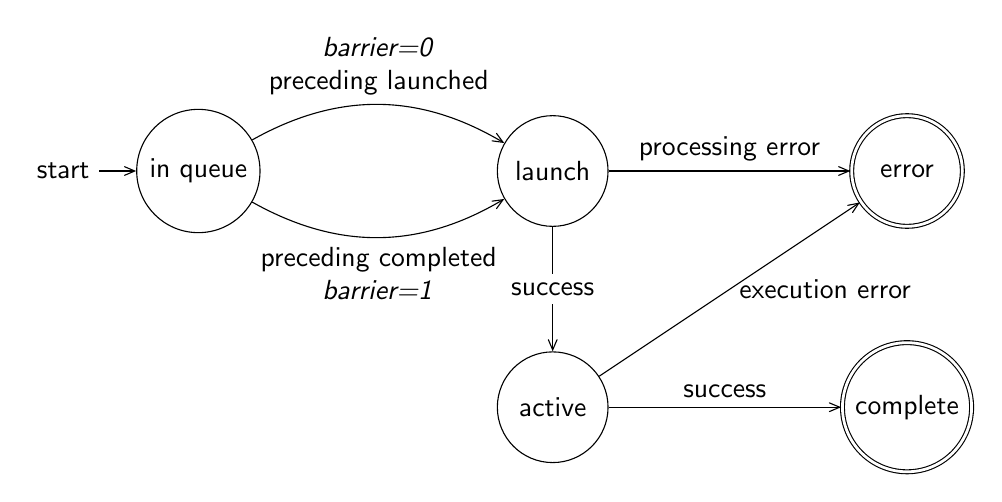
\begin{tikzpicture}
[auto,on grid,node distance=4.5cm,state/.style={circle,draw,minimum size=40pt}]
   \node[state,initial]                 (s0) {in queue};
   \node[state,right=4.5cm of s0]       (s1) {launch};
   \node[state,below=3cm of s1]       (s2) {active};
   \node[state,accepting,double distance=1pt,right=of s1]   (s3) {error};
   \node[state,accepting,double distance=1pt,right=of s2]   (s4) {complete};
   \path[->]
     (s0) edge[bend right]  node[text width=3cm,align=center,below] {preceding completed\\\textit{barrier=1}} (s1)
          edge[bend left] node[text width=3cm,align=center,above]{\textit{barrier=0}\\preceding launched} (s1)
     (s1) edge  node {processing error} (s3)
          edge  node[anchor=center,fill=white,opacity=1] {success} (s2)
     (s2) edge  node{success} (s4)
          edge  node[right]{execution error} (s3)
     ;
\end{tikzpicture}
  \centering
  \caption{Packet State Diagram}
  \label{fig:packetstate}
\end{figure}

\begin{description}[itemsep=2pt,leftmargin=0cm, labelindent=0cm]
\item[In queue] The packet processor has not started to parse the current
  packet.  The transition to the launch state only occurs after all the
  preceding packets have completed their execution if the \reffld{barrier} bit
  is set in the header. If the bit is not set, the transition occurs after the
  preceding packets have finished their launch phase. In other words, while the
  packet processor is required to launch any consecutive two packets in order,
  it is not required to complete them in order unless the barrier bit of the
  second packet is set.

\item[Launch] The packet is being parsed, but it did not start executing. This
  phase finalizes by applying an acquire memory fence with the scope indicated
  by the \reffld{acquire_fence_scope} header field.  Memory fences are discussed
  in~\cite{prm}, Section 6.2.6.

  If an error is detected during launch, the queue transitions to the error
  state and the event callback associated with the queue (if present) is
  invoked. The runtime passes a status code to the callback that indicates the
  source of the problem.  The following status codes might be returned:
  \begin{description}[itemsep=1.5pt,labelindent=.5cm]
  \item[\hsaref{HSA_STATUS_ERROR_INVALID_PACKET_FORMAT}] Malformed AQL
    packet. This could happen if, for example, the packet header type is invalid.
  \item[\hsaref{HSA_STATUS_ERROR_OUT_OF_RESOURCES}] The packet processor is
    unable to allocate the resources required by the launch. This could happen
    if, for example, a Dispatch packet requests more group memory than the size
    of the group memory declared by the corresponding component.
  \end{description}
\item[Active] The execution of the packet has started.

  If an error is detected during this phase, the queue transitions to the error
  state, a release fence is applied to the packet with the scope indicated by
  the \reffld{release_fence_scope} header field, and the completion signal (if
  present) is assigned a negative value. There is no invocation of the callback
  associated with the queue.

  If no error is detected, the transition to the complete state happens when the
  associated task finishes (in the case of Dispatch and Agent Dispatch packets),
  or when the dependencies are satisfied (in the case of a Barrier packet).

\item[Complete] A memory release fence is applied with the scope indicated by
  the \reffld{release_fence_scope} header field, and the completion signal (if
  present) decremented.

\item[Error] An error was encountered during the launch or active phases. No
  further packets will be launched on the queue. The queue cannot be recovered,
  but only inactivated or destroyed. If the application passes the queue as an
  argument to any HSA function other than \hsaref{hsa_queue_inactivate} or
  \hsaref{hsa_queue_destroy}, the behavior is undefined.

\end{description}

\subsection{API}
\input{api/altlatex/group-aql}

\section{Memory}\label{sec:memory}

One of the key features of HSA is its ability to share global pointers between
the host application and code executing on any component in a coherent
fashion. An application can directly pass a buffer allocated on the host (for
example, using malloc) to a kernel dispatched in any component. Kernels might
also access memory that is not in the coherent, global segment.

The HSA runtime API provides a compact set of functions for inspecting
the memory \emph{regions} that are accessible from  an agent, and (if applicable)
allocating memory on those regions from the host.

A memory region represents a block of contiguous memory that is directly
accessible by an agent, and exposes properties about the block of memory and how
it is accessed from that particular agent. The same block of memory -virtual or
physical- might be accessible from multiple agents, but the runtime creates a
unique region on every agent to represent the memory block. The characteristics
of a memory region include its size, addressability, access speed, and
corresponding memory segment. One agent might be able to access multiple regions
within the same segment.

The function \hsaref{hsa_agent_iterate_regions} can be used to inspect the set
of regions associated with an agent. Implementations of
\hsaref{hsa_agent_iterate_regions} are required to report the following
regions on every agent:
\begin{itemize}[itemsep=1pt,topsep=3pt,partopsep=0pt]
\item A region that starts at address 0, and is located in the global
  segment. This corresponds to the coherent, primary HSA memory type. All the
  regions with these characteristics should have identical sizes.
\item A region that is located in the global segment and can be used to allocate
  backing storage for the kernarg segment: \hsaref{HSA_REGION_FLAG_KERNARG} is
  true, and \hsaref{HSA_REGION_INFO_ALLOC_MAX_SIZE} is not 0. All the regions
  with these characteristics should have identical sizes.
\end{itemize}

If the application can allocate memory in a region using
\hsaref{hsa_memory_allocate}, the value of the attribute
\hsaref{HSA_REGION_INFO_ALLOC_MAX_SIZE} is different from zero. The runtime
allocator can only be used to allocate memory in the global segment. Memory in
the private, group and kernarg segments is automatically allocated when a
Dispatch packet is launched.

When the application no longer needs a buffer allocated using
\hsaref{hsa_memory_allocate}, it invokes \hsaref{hsa_memory_free} to release the
memory. The application shall not release a runtime-allocated buffer using
standard libraries (for example, free). Conversely, the runtime deallocator
cannot be used to release memory allocated using standard libraries (for
example, malloc).

If a buffer created in the host is also accessed by a component, applications
are encouraged to \emph{register} the corresponding address range beforehand
using the \hsaref{hsa_memory_register} function. While kernels running on HSA
components can access any regular host pointer, a registered buffer might
result on improved access performance.  When the application no longer needs to
access a registered buffer, it should deregister that virtual address range by
invoking \hsaref{hsa_memory_deregister}.

\subsection{Example - passing arguments to a kernel}\label{ex:kernarg_dispatch}
In the kernel setup example listed in Section~\ref{dispatch-packet}, the kernel
receives no arguments:
\begin{lstlisting}
// Indicate which ISA to run. The application is expected to have finalized a kernel (for example, using the finalization API).
// We will assume that the kernel object location is stored in KERNEL_ADDRESS
dispatch_packet->kernel_object_address = (uint64_t) KERNEL_ADDRESS;

// Assume our kernel receives no arguments.
dispatch_packet->kernarg_address = 0;
\end{lstlisting}
Let's assume now that the kernel expects a single argument, a signal handle. The
application needs to populate the \reffld{kernarg_address} field of the Dispatch
packet with the address of a buffer containing the signal.

The application searches for a memory region that can be used to allocate
backing storage for the kernarg segment. Once found, it reserves enough space to
hold the signal argument. While the actual amount of memory to be allocated is
determined by the finalizer, for simplicity we will assume that it matches the
natural size of the signal type, 8 bytes.
\begin{lstlisting}
// Indicate which ISA to run. The application is expected to have finalized a kernel (for example, using the finalization API).
// We will assume that the kernel object location is stored in KERNEL_ADDRESS
dispatch_packet->kernel_object_address = (uint64_t) KERNEL_ADDRESS;

hsa_region_t region;
hsa_agent_iterate_regions(component, get_kernarg, &region);
hsa_memory_allocate(region, 8, (void**) &dispatch_packet->kernarg_address);
\end{lstlisting}

, where the definition of \textit{get_kernarg} is:
\lstinputlisting[firstline=50, lastline=60]{example/kernarg_dispatch.c}

Finally, the application stores a signal handle in the buffer.
\begin{lstlisting}
hsa_signal_t* buffer = (hsa_signal_t*) dispatch_packet->kernarg_address;
assert(buffer != NULL);
hsa_signal_t signal;
hsa_signal_create(1, 1, &component, &signal);
*buffer = signal;
\end{lstlisting}
The rest of the dispatch process remains the same.

\subsection{API}
\input{api/altlatex/group-memory}

% \hypertarget{agent}{}\section{Agent Dispatch}\label{agent}
% The core runtime supports agent dispatches from an HSA agent. The
% runtime defines a default service queue for every user mode queue created by the
% user. This default service queue is available to the HSAIL programs and the user
% applications may submit agent dispatch packets to the service queue or any user
% mode queue. The service queue shares the same structure as the regular HSA
% queue. The default service queues are monitored by the
% runtime.

% \subsection{API}
% \input{api/altlatex/group-agent-dispatch}


\section{Extensions to the Core Runtime API}\label{extensions}

Extensions to the Core API can be optional (multi-vendor) or vendor
specific. The difference is in the naming scheme used for the symbols (defines,
structures, functions, etc.) associated with the function:

\begin{itemize}
\item Symbols for multi-vendor extensions defined in the global namespace must
  use the \emph{hsa_ext_} prefix in their identifiers.
\item Symbols for single vendor extensions defined in the global namespace must
  use the \emph{hsa_svext_VENDOR_} prefix in their identifiers. Company names
  must be registered with the HSA Foundation, must be unique, and may be
  abbreviated to improve the readability of the symbols.
\end{itemize}

Any constant definitions in the extension (\#define or enumeration values) use
the same naming convention, except using all capital letters.

The symbols for all vendor extensions (both single-vendor and multi-vendor) are
captured in the file {\bf hsa/vendor_extensions.h}. This file is maintained by
the HSA Foundation. This file includes the enumeration \hsaref{hsa_extension_t}
which defines a unique code for each vendor extension and multi-vendor
extension. Vendors can reserve enumeration encodings through the HSA
Foundation. Multi-vendor enumerations begin at the value of
\hsaref{HSA_EXT_START}, while single-vendor enumerations begin at
\hsaref{HSA_SVEXT_START}

\subsection{API}
\input{api/altlatex/group-extensions}

\subsection{Example}
An example that shows a hypothetical single-vendor extension ``Foo'' registered
by company ``ACME''. The example includes four defines and two API functions.
Note the use of the structure \reftyp{hsa_svext_acme_foo_t} and how this
interacts with the \hsaref{hsa_vendor_extension_query} API call.

\lstinputlisting{example/extension.c}

\section{Common Definitions}\label{sec:other}
\subsection{API}
\input{api/altlatex/group-common}
%\input{api/altlatex/group-clock}


\chapter{HSA Extensions Programming Guide}

\section{HSAIL Finalization}\label{sec:finalizer}

The Finalizer Core API is used to finalize given kernels and/or indirect
functions.  The Finalizer Core API is a vendor-specific low-level API. It can be
used to generate code for kernels and indirect functions from a specific program
for a specific HSA component using \hsaref{hsa_ext_finalize}. A kernel can only
be finalized once per program per agent. An indirect function can only be
finalized once per program per agent per call convention. Only code for the HSA
components specified when the program was created can be requested.

The program must contain a definition for the requested kernels and indirect
functions amongst the modules that have been added to the program. The modules
of the program must collectively define all variables, fbarriers, kernels and
functions referenced by operations in the code block of:
\begin{itemize}
\item{The kernel and indirect functions being finalized.}
\item{The transitive closure of all functions specified by call or scall
operations starting with the kernel and indirect functions being finalized.
Refer to the HSA Programmer's Reference Manual~\cite{prm}, Chapter 10 for
Function Operations.}
\end{itemize}

When invoking the finalizer, one or more kernels and indirect functions can be
requested. Requested kernels and indirect functions are represented as an
array of \hsaref{hsa_ext_finalization_request_t}. On some implementations
specifying multiple kernels and indirect functions can produce code with better
performance than finalizing the kernels and indirect function individually. For
example, it can allow the finalizer to generate common code for shared functions
which can reduce code footprint and improve instruction cache performance.

The Finalizer Core API allocates a kernel descriptor for every kernel definition
in a program, and an indirect function descriptor for every indirect function
definition in the program. Both kinds of descriptors are represented as an array
of \hsaref{hsa_ext_code_descriptor_t} in global segment memory. Each code
descriptor provides the information about a finalization of the kernel or
indirect function for a specific HSA component, and for indirect functions, a
specific call convention of that HSA component. An HSA runtmie uses an array of
finalization handles \hsaref{hsa_ext_finalization_handle_t} to access code
descriptors.

The kernel descriptor array is indexed by the agent id
\hsaref{hsa_ext_program_agent_id_t} The kernel descriptor and agent id are
available by the \emph{ldk} and \emph{agentid} operations respectively, or by an
HSA runtime queries \hsaref{hsa_ext_query_kernel_descriptor_address} and
\hsaref{hsa_ext_query_program_agent_id}. Refer to the HSA Programmer's Reference
Manual~\cite{prm}, Chapter 4.2.1 for Agent Id and 11.3 for User Mode Queue
Operations.

The indirect function descriptor is indexed by the call convention id
\hsaref{hsa_ext_program_call_convention_id32_t} which is performed implicitly by
the \emph{icall} operation. The indirect function descriptor address is
available by the \emph{ldi} operation or an HSA runtime query
\hsaref{hsa_ext_query_indirect_function_descriptor_address}. Refer to the HSA
Programmer's Reference Manual~\cite{prm}, Chapter 4.2.2 for Call Convention Id
and 10.8 for Indirect Call (icall, ldi) Operations.

The finalizer updates the code descriptor corresponding to the agent or call
convention for each kernel or indirect function that it finalizes.

The layout of a \hsaref{hsa_ext_code_descriptor_t} is defined by the HSA runtime.
It includes a kind field \hsaref{hsa_ext_code_kind32_t} that indicates whether
the code descriptor contains finalized code. If it has been finalized, then for
kernels the information needed to create a User Mode Queue kernel dispatch
packet is available, including:
\begin{itemize}
\item{The byte size of the group segment for a single work-group:}
  \subitem{Includes module scope and function scope group segment variables used
    by the kernel or any functions it calls directly or indirectly.}
  \subitem{Includes any finalizer allocated temporary space. For example, in the
    implement of exception operations or fbarriers.}  \subitem{Does not include
    any dynamically allocated group segment space. Refer to the HSA Programmer's
    Reference Manual~\cite{prm}, Chapter 4.20 Dynamic Group Memory Allocation}
\item{The byte size of the private segment for a single work-item. This
    includes:} \subitem{Module scope and function scope private segment
    variables.}  \subitem{Space for function scope spill segment variables
    allocated in memory} \subitem{Space for argument scope arg segment variables
    allocated in memory.}  \subitem{Any space needed for saved HSAIL or ISA
    registers due to calls.}  \subitem{Any other finalizer introduced
    temporaries including spilled ISA registers and space for function call
    stack.}
\item{The 64-bit opaque code handle to the finalized code that includes the
    executable ISA for the HSA component. It can be used for the kernel dispatch
    packet kernel object address field.}
\end{itemize}

The code descriptor also includes other information that may be useful to a
high-level language runtime to invoke and manage the kernel's execution. For
example, the size and alignment of the kernarg segment and the call convention
used by the code of the kernel.

For an indirect function, a code descriptor includes:
\begin{itemize}
\item{The 64-bit opaque code handle to the finalized code that includes the
    executable ISA for a single call convention of the HSA component.}
\end{itemize}

Once code has been generated for a kernel for a specific HSA component, it can
be executed by adding a kernel dispatch packet to a User Mode Queue associated
with the HSA component. The information required to create the kernel dispatch
packet is available in the code descriptor addressed by using the agent id to
index the kernel descriptor.

For an indirect function, the code is only made available to kernel dispatches
launched after the indirect function has been finalized. Therefore, prior to
executing a kernel, all indirect functions that it will call must have been
finalized for the HSA component with the call convention used by the kernel
code. The \emph{icall} operation, used to call indirect functions, implicitly
access the code descriptor addressed by using the call convention id of the
executing kernel to index the indirect function descriptor. Refer to the HSA
Programmer's Reference Manual~\cite{prm}, Chapter 4.2.2 for Call Convention Id
and 10.8 for Indirect Call (icall, ldi) Operations.

Appropriate memory synchronization is needed to access the code descriptor since
it is updated concurrently by the HSA runtime. Memory synchronization may
include using an acquire fence at system scope on the kernel dispatch packet if
the code descriptor may have changed since the HSA component executed the last
packet acquire fence at system scope, or using a load acquire at system scope on
the code descriptor kind field if the code descriptor may change during the
execution of the kernel dispatch. This applies both to accesses performed
explicitly to create kernel dispatch packets, and implicitly by the \emph{icall}
operation.

The code will remain available to execute until the HSA runtime is used to
destroy the HSAIL program with which the code is associated using
\hsaref{hsa_ext_program_destroy}. All HSAIL programs created by the application
are implicitly destroyed when the application terminates.

\subsection{API}
\input{api/altlatex/group-ext-finalizer}

%\subsection{Group Memory Usage}\label{groupmem}

% Group memory can be allocated either
% statically when the finalizer is called or dynamically by the user at launch
% time.

% Static allocation is supported as follows:
% \begin{itemize}
% \item The \hsaref{hsa_finalize_brig} routine writes the amount of group memory
%   needed by the finalized ISA to the
%   \hsaref{hsa_code_descriptor_t}.\reffld{workgroup_group_segment_size_byte}
%   field. The group memory usage includes group memory which is statically
%   allocated in the HSAIL kernel, as well as private group memory used by the
%   finalizer. Different HSA implementations might allocate different amounts of
%   group memory.

% \item The user copies the requested group segment usage to the Dispatch packet
%   field \reffld{group_segment_size_bytes}.

% \item The packet processor reads the group memory usage field and reserves the
%   required resources at dispatch time.

% \item Statically allocated group memory starts at a segment offset of 0.

% \end{itemize}

% Dynamically allocated group memory allows the user to specify the group memory
% size when the kernel is launched. This is useful to support dynamic group memory
% allocation features supported by languages such as OpenCL. Essentially, the user
% manually calculates the offset for each kernel argument (including the static
% allocation in the calculation) and passes these as arguments to the HSAIL
% kernel. Specifically:

% \begin{itemize}

% \item As above, the \hsaref{hsa_finalize_brig} routine returns the requested
%   static group allocation.

% \item HSAIL will use standard 32-bit arguments (that is, \ttbf{kernarg_u32})
%   to specify group segment offsets. The user is responsible for computing the
%   offset for each group memory argument location. The first argument must start
%   just above the static allocation, so it always has the offset of
%   \reffld{workgroup_group_segment_size_byte} (see
%   \hsaref{hsa_code_descriptor_t}).

% \item After setting the offset for each group memory argument, the user must set
%   the AQL Dispatch packet's \hsaref{hsa_aql_dispatch_packet_t}.\reffld{
%     group_segment_size_bytes} field to the total amount of group memory used
%   (static and dynamic allocations).

% \end{itemize}

% See below for an example of setting up dynamic group memory arguments for a
% kernel.  \lstinputlisting{example/group-sample.c}

% Here is the corresponding kernel and usage model:
% \lstinputlisting{example/group-sample-hsail.c}

\section{HSAIL Linking}\label{linking}

HSAIL Linker Service Layer is vendor-neutral high level API that provides
semantics for HSAIL inter-module linking. Linking between modules is done within
the context of the HSAIL program.

An application can use the HSA runtime to create zero or more HSAIL programs
using \hsaref{hsa_ext_program_create}. Created HSAIL programs can be accessed
through \hsaref{hsa_ext_program_handle_t}, which is returned from the program
creation call.  When the program is created, one or more HSA components
\hsaref{hsa_agent_t} that are part of HSA platform must be specified, together
with the machine model \hsaref{hsa_ext_brig_machine_model8_t} and profile
\hsaref{hsa_ext_brig_profile8_t}.

The set of agents associated with a program cannot be changed after it has been
created. Within a program, each of these HSA component members has a unique
identifier \hsaref{hsa_ext_program_agent_id_t} in the range 0 to the number of
agent members minus one. The same HSA component may have a different agent
identifier in different HSAIL programs that it is a member. In addition, each
HSA component can support one or more call conventions
\hsaref{hsa_ext_program_call_convention_id32_t}. For example, an HSA component
may have different call conventions that each use a different number of isa
registers to allow different numbers of wavefronts to execute on a compute unit.
When the HSA runtime is used to create an HSAIL program, it determines a dense
call convention id ordering for the program. The first agent is assigned call
convention ids 0 to the number of call conventions it supports minus one.  The
next agent is assigned the next range of call conventions according to the
number it supports, and so on. Note that the same agent may have a different
range of call convention ids in different programs of which it is a member. An
HSA runtime query \hsaref{hsa_ext_query_call_convention} is available to
determine the range of call convention ids used for a particular agent of a
particular program.

The machine model address size for the global segment must match the size used
by the application.

An application can add zero or more HSAIL modules \hsaref{hsa_ext_brig_module_t}
to the HSAIL program using \hsaref{hsa_ext_add_module}. HSAIL module is the unit
of HSAIL generation, and can contain multiple symbol declarations and
definitions. Distinct instances of the symbols it defines are created within
each program, and symbol declarations are only linked to the definitions
provided by other modules in the same program. The same HSAIL module can be
added to multiple HSAIL programs, which allows multiple instances of the same
kernel and indirect functions that reference distinct allocations of global
segment variables.  The same HSAIL module cannot be added to the same HSAIL
program more than once. The machine model and profile of the HSAIL module that
is being added has to match the machine model and profile of the HSAIL program
it is added to. HSAIL modules and their handles can be queried from the program
using several query operations, for example
\hsaref{hsa_ext_query_program_modules} queries specified number of module
handles, \hsaref{hsa_ext_query_program_brig_module} queries module with
specified module handle. HSAIL modules contained in the program can be accessed
through the module handle \hsaref{hsa_ext_brig_module_handle_t}.

Linker Service Layer manages linking of symbol declarations to symbol
definitions between modules, therefore the low\-level APIs can request certain
definitions and addresses using \hsaref{hsa_ext_symbol_definition_callback_t}
and \hsaref{hsa_ext_symbol_address_callback_t} respectively. In addition, the
application can provide symbol definitions to an HSAIL program using
\hsaref{hsa_ext_define_agent_allocation_global_variable_address} and
\hsaref{hsa_ext_define_readonly_variable_address}, and request the address of
symbols defined by the HSAIL program using
\hsaref{hsa_ext_query_symbol_definition},
\hsaref{hsa_ext_query_program_allocation_global_variable_address},
\hsaref{hsa_ext_query_agent_global_variable_address},
\hsaref{hsa_ext_query_readonly_variable_address}.

Once the program is linked and finalized, it is application's responsibility to
destroy the program. Destroying the program will deallocate all code objects, so
the code will become unavailable.

\subsection{API}
\input{api/altlatex/group-ext-linker}


\section{Images and Samplers}\label{images}

An HSA runtime uses an image handle \hsaref{hsa_ext_image_handle_t} to access
images. The image handle references the image data in memory and records
information about resource layout and other properties. HSA decouples the
storage of the image data and the description of how the device interprets that
data. This allows the application developer to control the location of the
image data storage and manage memory more efficiently.

The HSA image format is specified using a format descriptor
(\hsaref{hsa_ext_image_format_t}) that contains information about the image
channel type and the channel order. The image channel type describes how the
data is to be interpreted along with the bit size, and image channel order
describes the number and the order. Not all image channel types and channel
order combinations are valid on a HSA agent. All HSA agents have to support a
required minimum set of image formats. For more information, refer to the HSA
Programmer's Reference Manual\cite{prm}. An application can use
\hsaref{hsa_ext_image_get_format_capability} to query a runtime
to obtain image format capabilities.

An implementation-independent image format descriptor
(\hsaref{hsa_ext_image_descriptor_t}) is composed of geometry along with the
image format. The image descriptor is used to inquire the runtime for the HSA
component-specific image data size and alignment details by calling
\hsaref{hsa_ext_image_get_info} for the purpose of determining the
implementation's storage requirements.

The memory requirements (\hsaref{hsa_ext_image_info_t}) include the size of the
memory needed as well as any alignment constraints. An application can either
allocate new memory for the image data, or sub-allocate a memory block from an
existing memory if the memory size allows. Before the image data is used, an HSA
agent-specific image handle must be created using it and if necessary, cleared
and prepared according to the intended use.

A HSA agent-specific image handle (\hsaref{hsa_ext_image_handle_t}) is used by
the HSAIL language for reading or writing using HSAIL \refhsl{rd image},
\refhsl{ldimage} and \refhsl{stimage}
operations. \hsaref{hsa_ext_image_create_handle} creates an image handle from a
implementation-independent image format descriptor and independently allocated
image data that conforms to the requirements provided by
\hsaref{hsa_ext_image_get_info}.

It must be noted that while the image data technically accessible from its
pointer in the raw form, the data layout and organization is agent-specific and
should be treated as opaque. The internal implementation of an optimal image
data organization could vary depending on the attributes of the image format
descriptor. As a result, there are no guarantees on the data layout when
accessed from another HSA agent. The only reliable way to import or export image
data from optimally organized images is to copy their data to and from a
linearly organized data layout in memory, as specified by the image's format
attributes.

The HSA runtime provides interfaces to allow operations on images. Image data
transfer to and from memory with a linear layout can be performed using
\hsaref{hsa_ext_image_export} and \hsaref{hsa_ext_image_import} respectively. A
portion of an image could be copied to another image using
\hsaref{hsa_ext_image_copy}. An image can be cleared using
\hsaref{hsa_ext_image_clear}. It is the application's responsibility to ensure
proper synchronization and preparation of images on accesses from other image
operations. See HSA System Architecture spec 2.13 for the HSA Image memory
model.

A HSA agent-specific sampler handle (\hsaref{hsa_ext_sampler_handle_t}) is used
by the HSAIL language to describe how images are processed by the
\refhsl{rdimage} HSAIL operation. \hsaref{hsa_ext_sampler_create_handle} creates
a sampler handle from an agent independent sampler descriptor
(\hsaref{hsa_ext_sampler_descriptor_t}).

\subsection{API}
\input{api/altlatex/group-ext-images}

% \section{Component Initiated Dispatches} \label{architected}

% Due to architected support for a queue and design of AQL, HSA supports
% component-initiated dispatch, which is the ability for a kernel to dispatch a
% new kernel by writing an AQL packet directly to a user queue. In simple use
% cases, the AQL packet can be created on the host and passed as a parameter to
% the kernel. This eliminates the need to do dynamic memory allocation on the
% component, but has the limitation that the problem fanout must be known at the
% time the first kernel is launched (so that the AQL packets can be
% preallocated). HSA also supports more advanced use cases where the AQL packet is
% dynamically allocated (including the memory space for kernel arguments and
% spill/arg/private space) on the component. This usage model obviously requires
% dynamic component-side memory allocation, for both host and component memory.

% Some requirements to do component-initiated dispatch:
% \begin{itemize}
% \item Ability to dynamically choose a kernel to dispatch: Let us assume for
%   example that there are three kernels (A, B and C). If the host launches A,
%   then the user has the choice of launching B or C, or even A in case of
%   recursion. So, the user should be able to get the ISA and segment size
%   (Hsa\-Aql\-Kernel) from the corresponding BRIG dynamically. \mbox{[}caveat:
%   The code sample here does not show how we can do this. It assumes that the
%   Hsa\-Aql\-Kernel is being passed as an argument to the parent kernel (A in
%   this case)\mbox{]}

% \item Ability to dynamically allocate memory from the shader: We need to
%   allocate memory for AQL\-Packet, different kernel segments in the AQL\-Packet,
%   kernel arguments, and so forth.

% \item Ability for a finalizer to identify a default HSA queue to write
%   AQL\-Packet: The HSA queue information resides in the runtime layer of the
%   stack. This needs to be exchanged with the compiler so it can be stored in the
%   global space. This way, when the compiler sees the queue, it knows where to
%   pick the HSA queue information to write the AQL-Packet.

% \item Ability to notify the completion of all the component-initiated
%   dispatches on the host:

% \begin{itemize}
% \item The beginning of execution of the child kernel may or may not wait for the
%   parent kernel's completion. This is determined by the user and could be
%   algorithm dependent.
% \item If the parent (initiated from host) kernel finishes successfully, it means
%   all kernels it initiated also finished successfully.
% \item To implement this, we need to track the list of kernels launched from the
%   parent. Change the status of parent to complete, only if parent and all its
%   child kernels have completed successfully.
% \end{itemize}
% \end{itemize}

% Implementations that support component initiated dispatches will need to support
% these requirements. If the implementation supports the stated requirements, the
% following actions will allow a component to initiate a dispatch:
% \begin{itemize}
% \item The queue and \hsaref{hsa_ext_code_descriptor_t} (describing the kernel to
%   launch) can be passed as arguments to the parent (the one launched from the
%   host) kernel. If the dispatch is to the same queue, it is accessible via an
%   HSAIL instruction.
% \item If not, get the Hsa\-Aql\-Kernel from the BRIG for the kernel that is
%   chosen to be dynamically dispatched.
% \item When new work is to be created, the HSAIL code would:
% \begin{itemize}
% \item Use the kernel dynamic memory allocator to allocate a new AQL\-Packet.
% \item Use inline HSAIL to replicate the functionality of the
%   Hsa\-Init\-AQL\-Packet function. We could perhaps provide an HSAIL library to
%   implement this functionality. Recall this function:
% \begin{itemize}
% \item Copies some fields from the Hsa\-Aql\-Kernel structure (for example, the
%   kernel ISA) to the AQL\-Packet
% \item Uses a host allocator to allocate memory for the kernel arguments
% \item Uses a component allocator to allocate memory for spill, private, and arg
%   segments
% \end{itemize}
% \end{itemize}
% \item The HSAIL knows the signature of the called function and can fill in the
%   AQL packet with regular HSAIL global store instructions.
% \item The HSA queue is architected, so the HSAIL can use memory store
%   instructions to dispatch the kernel for dispatch. Depending how the user
%   queues are configured, atomic accesses might be necessary to handle contention
%   with other writers. Note that, if the queue information is not passed in as an
%   argument, the default queue can be chosen by the finalizer as it was exchanged
%   earlier from the runtime layer.
% \item We also need to handle deallocation of the kernel arguments and
%   spill/private/arg space after the kernel completes.
% \item On the host, check if the parent has finished. If the parent has finished
%   successfully, then it means that all the child kernels have finished
%   successfully too. If the parent or any of the child kernels failed, an error
%   code will be returned.
% \end{itemize}

% Glossary

\appendix
\chapter{Glossary}
\begin{description}[itemsep=5pt,leftmargin=0cm, labelindent=0cm]

\item[Architected Queuing Language (AQL)] A command interface for the dispatch
  of HSA Agent commands.

\item[Arg segment] A memory segment used to pass arguments into and out of
  functions.

\item[BRIG] The HSAIL binary format.

\item[Compute unit] A piece of virtual hardware capable of executing the HSAIL
  instruction set. The work-items of a work-group are executed on the same
  compute unit. An HSA component is composed of one or more compute units.

\item[Finalizer] A back-end compiler that translates HSAIL code into native ISA
  for a compute unit.

\item[Global segment] A memory segment in which memory is visible to all
  work-items in all HSA components and to all host CPUs.

\item[Grid] A multidimensional, rectangular structure containing work-groups. A
  Grid is formed when a program launches a kernel.

\item[Group segment] A memory segment in which memory is visible to a single
  work-group.

\item[Host CPU] An HSA Agent that also supports the native CPU instruction set
  and runs the host operating system and the HSA runtime. As an HSA Agent, the
  host CPU can dispatch commands to an HSA Component using memory operations to
  construct and enqueue AQL packets. In some systems, a host CPU can also act as
  an HSA Component (with appropriate HSAIL finalizer and AQL mechanisms).

\item[HSA Agent] A hardware or software component that participates in the HSA
  memory model. An HSA Agent can submit AQL packets for execution. An HSA Agent
  may also but is not required to be an HSA Component. It is possible for a
  system to include HSA Agents that are neither HSA Components nor host CPUs.

\item[HSA application] A program written in the host CPU instruction set
  architecture (ISA). In addition to the host CPU code, it may include zero or
  more HSAIL programs.

\item[HSA Component] An HSA Agent that supports the HSAIL instruction set and
  the AQL packet format. As an HSA Agent, an HSA Component can dispatch commands
  to any HSA Component (including itself) using memory operations to construct
  and enqueue AQL packets. An HSA Component is composed of one or more compute
  units.

\item[HSA implementation] A combination of (1) hardware components that execute
  one or more machine instruction set architectures (ISAs), (2) a compiler,
  linker, and loader, (3) a finalizer that translates HSAIL code into the
  appropriate native ISA if the hardware components cannot support HSAIL
  natively, and (4) a runtime system.

\item[HSA Packet Processor] HSA Packet Processors are tightly bound to one or
  more HSA Agents, and provide the user mode queue functionality for the HSA
  Agents. HSA Packet Processors participate in the HSA memory model and are HSA
  Agents.

\item[HSA runtime] A library of services that can be executed by the application
  on a host CPU that supports the execution of HSAIL programs. This includes a
  finalizer that translates HSAIL code into the appropriate native ISA for each
  HSA component that is part of the HSA system. In additional, it supports a
  runtime queue that can be used by any agent, including HSA components, to
  submit agent dispatch packets to perform runtime functions.

\item[HSAIL] Heterogeneous System Architecture Intermediate Language. A virtual
  machine and a language. The instruction set of the HSA virtual machine that
  preserves virtual machine abstractions and allows for inexpensive translation
  to machine code.

\item[Image handle] An opaque handle to an image that includes information about
  the properties of the image and access to the image data.

\item[Kernarg segment] A memory segment used to pass arguments into a kernel.

\item[Kernel] A section of code executed in a data-parallel way by an HSA
  Component. Kernels are written in HSAIL and then separately translated by a
  finalizer to the target instruction set.

\item[Packet ID] Each AQL packet has a 64-bit identifier unique to the queue
  scope. The identifier is assigned as the sequential number of the packet slot
  allocated in the queue.

\item[Private segment] A memory segment in which memory is visible only to a
  single work-item. Used for read-write memory.

\item[Readonly segment] A memory segment for read-only memory.

\item[Sampler handle] An opaque handle to a sampler which specifies how
  coordinates are processed when an image is read within a kernel.

\item[Segment] A contiguous addressable block of memory. Segments have size,
  addressability, access speed, access rights, and level of sharing between
  work-items. Also called memory segment.

\item[Signal (handle)] An opaque handle to a signal which can be used for
  notification between threads and work-items belonging to a single process
  potentially executing on different agents in the HSA system.

\item[Spill segment] A memory segment used to load or store register spills.

\item[Wavefront] A group of work-items that share a single program counter.

\item[Work-group] A collection of work-items.

\item[Work-item] The simplest element of work.

\end{description}

% API index
% the combination of page break  + \markboth sets \rightmark \leftmark to a
% value different from that of the previous Chapter and Section.
\newpage
\markboth{Index - APIs}{Index - APIs}
\printindex[api]
\printindex[ext]

% inline bibliography for simplicity.
\bibliographystyle{plain}
\begin{thebibliography}{30}

\bibitem{prm}
\newblock{HSA Programmer's Reference Manual.}
\newblock{Provisional 1.0 - Ratified, HSA Foundation, 2014/06/05.}

\bibitem{sar}
\newblock{HSA Platform System Architecture Specification.}
\newblock{Provisional 1.0 - Ratified, HSA Foundation, 2014/04/18.}

\end{thebibliography}
% add bibliography to Table of Contents
\addcontentsline{toc}{chapter}{Bibliography}

\end{document}

%  LocalWords:  incrementing allocators enqueuing
